\documentclass{article}
\usepackage{tikz}
\usetikzlibrary{arrows}

\begin{document}
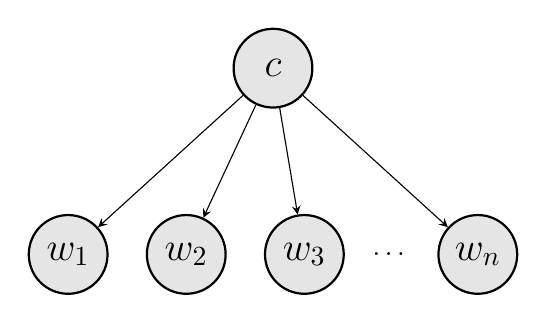
\begin{tikzpicture}[->,>=stealth, auto, main node/.style={thick, circle, draw, minimum size=1cm, font=\sffamily\Large, fill=black!10, node distance=2.5cm, shorten >=1pt}, every node/.style={thick, node distance=2.5cm}]
\node [main node] {$c$}
child{ node [main node, left=10pt, below=10pt] {$w_1$} }
child{ node [main node, left=10pt, below=10pt] {$w_2$} }
child{ node [main node, left=10pt, below=10pt] (1) {$w_3$} }
child{ node [main node, right=10pt, below=10pt] (2) {$w_n$} };

\path (1) -- node[auto=false]{\ldots} (2);
;
\end{tikzpicture}
\end{document}